\section{Collaborative Research: Theory of computation in cell cultured neural networks}
\section{Section 1: Contact information for the Israeli PI}
\noindent Prof. Elisha Moses, Weizmann Institute of Science, +917-8-934-3139, \href{mailto:elisha.moses@weizmann.ac.il}{elisha.moses@weizmann.ac.il}
%\begin{tabular}{ l l }
%Prof. Elisha Moses & Prof. Aviv Bergman\\
%Physics of Complex Systems & Department of Systems and Computational Biology\\
%Weizmann Institute of Science & Albert Einstein College of Medicine\\
%PO Box 26 & Price Center Rm. 153\\
%Rehovot 76100 & Bronx, NY 10461\\
%Israel & USA\\
%Phone +917-8-934-3139 & Phone +1-718-678-1063\\
%Email elisha.moses@weizmann.ac.il & Email aviv@einstein.yu.edu\\
%\end{tabular}

\section{Section 2: IOS Program Justification}
\label{sec:justification}
\noindent BIO/IOS Neural Systems NSF 11-572. Our proposed work is most appropriate for the IOS neural systems section as it deals with fundamental questions relating to the computational capabilities of the central nervous systems of living organisms. The associated questions we intend to address are fundamental to an integrative understanding of structure-function physiology and co-evolution in all organisms with nervous systems and the evolutionary predecessors that gave rise to them. With respect to nervous system \emph{organization}, we intend to deepen previous explorations into the interaction of developmental and environmental constraints on the architecture and complementary computational capacity of networks of living neurons. Focusing on flexible abstract models of computation, rather than those specific to digital electronics, will enable us to investigate potentially novel computational potential implemented via architectures that differ from digital electronics in their apparent ability to take advantage of synergy between stochastic and deterministic properties. We may therefore, in addition to contributing to fundamental biological understanding, identify computational principles unique to natural neural networks. It is essential in this project to link theoretical, computational and experimental methods of inquiry. This is necessary to address questions we ask regarding co-evolution and co-development between underlying biological organization and computational tasks such structures are capable of performing in a variety of environmental conditions. We have assembled a culturally diverse and interdisciplinary team of experienced and developing scientists to enable the success of the research program we propose.

\section{Section 3: Research description}

\subsection{Motivating questions}
One question regarding the brain is, why neurons that perform astoundingly complex calculations become inefficient at computation once they are grown outside of it. In particular, once one takes hippocampal neurons out of the rat brain and cultures them on a dish, they lose their individuality. Living neuronal cultures are characterized by all-or-none network bursts, where practically all the neurons fire simultaneously, with varying degrees of synchrony. While in the brain they can compute the trajectory of the animal in a maze, but as an ensemble grown out of it they seem unable to perform new computations, and can only carry very few bits of information \cite{Feinerman2006}. How is it then that individual neurons are organized in the brain as a splendid computer, but in the dish their computational repertoire seems limited? Obviously, their environment and growth conditions have changed, but can we isolate those elements that are necessary, and perhaps sufficient, to support computation by a living neuronal network? In an effort to tackle such questions, we have embarked on an investigation of the computational abilities of living neuronal networks, and propose here to expand this investigation both theoretically and experimentally.

On the conceptual side, a number of deep questions arise. What are the structural properties at the level of networks of neurons,
modules of networks of neurons, and perhaps higher order forms of
organization necessary to support the capacity for
abstraction, which is fundamental to computation \cite{Abelson1996} and may likewise be fundamental to
\href{http://en.wikipedia.org/wiki/Cognitive\_architecture}{cognitive
architecture}, development, and function \cite{Tenenbaum2011}? Given that we have shown boolean
logic devices capable of being implemented {\em in vitro} using
neurons \cite{Feinerman2008}, is it possible to biologically engineer analogous
devices capable of performing computations that have natural embeddings
within \href{http://en.wikipedia.org/wiki/First-order\_logic}{first} or
\href{http://en.wikipedia.org/wiki/Higher\_order\_logic}{higher-order
logic}?

We plan to experimentally develop a number of novel logical devices, as well as use a number of new technologies that we have acquired for the construction of such computational constructs. Notable among these are the optogenetic toolbox that has recently become available. Our access to this toolbox includes light induced neuronal excitation using channelrhodopsins (courtesy of the Deisseroth lab at Stanford and the Yizhar lab at Weizmann) as well as genetically encoded fluorescent labels for optical imaging of neuronal excitation (courtesy of the Cohen lab at Harvard).

Evolutionary forces have shaped the architecture, connectivity as well as the input that neurons grow with inside the brain, all of which are involved in its apparently emergent computational capability. Biological computation in general is set apart from that of electronic computers by the fact that the `hardware' (e.g. the cell or the organism) co-evolved with the `software' (DNA or the brain respectively). As a result, our `software' is naturally co-optimized for the associated `hardware', while in the computer world that is not necessarily, if ever, the case. This insight leads us to propose experiments that will connect the neuronal network with the `real' world, and  allow the structure and function to co-evolve in a range of different environmental conditions.

\subsection{\emph{Natural} models of computation in living neural networks}

Since the development of the electronic digital computer, which makes
use of the digital abstraction \cite{Ward1989} from analog electrical circuits
there has been a close heuristic association between boolean logic and
computation. However, developments in formal logic over the past century
have been largely motivated by its applications to computation and the
theory of programming languages that go beyond boolean logic to support additional forms of abstraction. The capacity to support abstraction mirroring various systems of
formal logic is the primary way in which languages are compared \cite{Abelson1996}. Electronic devices that are capable
of supporting such forms of abstraction provide a concrete physical
instantiation of the ideas inherent to the logical systems they are
designed to faithfully implement.

Neuronal logic devices (NLDs) represent an alternative physical modality
to digital electronics for the purpose of performing computation.
However, rather than attempting to directly parallel the history of the
development of digital electronics via the digital abstraction,
high-level descriptions of computation, such as the
$\lambda$-calculus, serve as a specification
of computation that is agnostic to the physical modality of
implementation. If the specification that a neuronal computation device
should be capable of implementing the
$\lambda$-calculus, which is Turing complete formal system, a natural first step
toward this broad goal is to investigate simple neuronal systems that
are capable of performing well-defined computations that require a
capacity for first- or some higher-order logic.

One challenge to be addressed experimentally is whether such a system can be implemented reliably using central nervous system (CNS) neurons, which are individually unreliable components. We have shown previously that complex devices such as a diode, an oscillator and an AND-gate can be engineered using CNS neurons grown on particular geometric configurations \cite{Feinerman2008}. While a complicated configuration of NAND gates could, in principle, enable the construction of a universal Turing machine, this may be difficult to engineer with previously developed methods. Alternative geometric configurations and measurement patterns coupled with developmental selection will enable the identification of configurations of neurons capable of performing more difficult computations.

To develop higher order computational devices, we will turn to the experimental techniques of microfluidics and optogenetics \cite{Yizhar2011,Kralj2012}.
It is now possible to monitor with optical means the electrical activity of the network without any collateral damage caused by the fluorescent dye. This is done by genetic incorporation of a fluorescent voltage-indicating protein into the neuron. It is furthermore possible to excite a region of the network optically by activating photosensitive channels that are genetically embedded as well. On top of this, the propagation velocity of a signal inside a one-dimensional neuronal network of the type we are using is constant, and can be reliably predicted. Thus it becomes possible to identify activity in one part of a device, and then excite another region co-incidentally with the arrival of the signal into that area. Different time delays, with the activation before, during or after the arrival of the synaptic input will allow the creation of several neuronal learning scenarios, and the comparison to learning in organisms with brains.

\subsection{A higher-order function to be implemented as a higher-order NLD}

The $\lambda$-calculus notation is helpful in
order to define any higher order function. This notation may be
implicitly familiar to users of imperative programming languages as ``anonymous functions''. We provide an informal set of examples necessary to clarify our work. Complete details can be found in \cite{Barendregt1985}. We can define a
standard binary boolean function like the ``and'' function as $\lambda x. \lambda y.(\wedge\,\,x\,\,y)$. Such a lambda expression can apparently be applied to any inputs;
however the inputs to such a function are not necessarily restricted to
booleans unless we infer that the standard logical operator
``$\wedge$'' only accepts boolean arguments.
Note that we have used the
\href{http://en.wikipedia.org/wiki/Polish\_notation}{prefix or Polish
notation} for the $\wedge$ operator, which
in the perhaps more common infix notation is written with its arguments
flanking the operator as $x \wedge y$ to mean
``$x$ and
$y$''. We can provide explicit type
annotations for the bound variables $x$
and $y$, which indicate the types of
the arguments $\lambda x:bool. \lambda y:bool.(\wedge\,\,x\,\,y)$. We can now also provide a type annotation for this expression as a whole
\begin{equation}\label{eq:boolfulltype}
[\lambda x:bool. \lambda y:bool.(\wedge\,\,x\,\,y)]:[bool \rightarrow bool \rightarrow bool]
\end{equation}
Depending upon conventions with respect to
\href{http://en.wikipedia.org/wiki/Currying}{currying}, one could read
the type annotation as ``the function that takes two arguments each of
type $bool$ and returns a values of type
$bool$'' or ``the function that takes an
argument of type $bool$ and returns a
function that takes an argument of type
$bool$ and returns a value of type
$bool$''. The first formulation may be
easier to read, but the second is standard as a result of the design of
functional programming languages.

Now we can imagine that if we wish to abstract from the particular
binary boolean function implied by the
$\wedge$ operator, we need to introduce a
functional variable, whose type will be explicitly denoted for
concreteness despite the fact that it could be inferred, for which this
operator can be substituted. Doing this results in the following second
order function
\begin{multline}\label{eq:lamhobf}
[\lambda f:(bool \rightarrow bool \rightarrow bool).
\lambda x:bool. \lambda y:bool.(f\,\,x\,\,y)]
\\
:[(bool \rightarrow bool \rightarrow bool)
\rightarrow bool \rightarrow bool \rightarrow bool]
\end{multline}
This function is intended to be read, in the less verbose uncurried
form, as ``the function that takes as its first argument, a function
that takes two boolean values as arguments and returns a boolean value,
and, as its second and third arguments, two boolean values, and returns a
boolean value''. It is perhaps remarkable that this simple abstraction
is now capable of implementing any of the 16 possible boolean functions,
provided that the proper binary boolean operator is submitted as the
first argument to this function. The statement of this
function in terms of $\lambda$-calculus is agnostic to any physical implementation capable of realizing extensionally
equivalent behavior.

To make this more concrete, we can very simply implement the above
function in any programming language.
An implementation in the programming language OCaml appears in listing \ref{camlhobf}.
\begin{lstlisting}[caption={a higher order boolean function},label=camlhobf]
let hobf = fun (bf : ('a 'a bool)) (i1 : bool) (i2 : bool)
	       -> bf i1 i2
\end{lstlisting}
What is required in order to evaluate this function are corresponding
implementations of boolean functions to be substituted either for
$f$ in the lambda calculus notation or
for bf in terms of the corresponding OCaml implementation. For example
we can implement the XOR function using pattern matching to define a
truth table as shown in listing \ref{camlXOR}.
\begin{lstlisting}[caption={implementation of an XOR boolean operator},label=camlXOR]
let xor p1 p2 = match (p1, p2)
with (false, false) -> false
   | (false,  true) -> true
   | ( true, false) -> true
   | ( true,  true) -> false
\end{lstlisting}
Other binary boolean functions are implemented in an analogous fashion.
In order to evaluate hobf we then simply provide the name of a binary
boolean function and two boolean values. For example $hobf \,\, xor \,\, 0 \,\, 0=0$ and $hobf \,\, xor \,\, 0 \,\, 1=1$.

\subsection{Assessment of abstraction potential in NLDs}
An important consideration is to state precisely some criterion for
determining that a particular NLD has achieved potential for an explicit
form of abstraction such as is indicated in the relationship between
expressions \ref{eq:boolfulltype} and
\ref{eq:lamhobf}. In abstracting the binary boolean
operator $\wedge$ to the functional variable
$f$, which is the fundamental
transformation enabling the derivation of
\ref{eq:lamhobf} from
\ref{eq:boolfulltype}, we imply that any physical
implementation must take at least three rather than two inputs and the
first of these must specify a particular binary boolean operator to
apply to the latter two boolean input values. This roughly means that
any system that at least partially implements the lambda expression or
function specified in equation \ref{eq:lamhobf} and
listing \ref{camlhobf} respectively , must be capable of
interpreting the concept of ``selection from a set'' whose size is
determined by the subset of the 16 binary boolean operators that is
already implemented in a lower-level form. Indeed another representation
of equation \ref{eq:lamhobf} as a partial or total
set function could be written as $hobf : Hex \times Bool \times Bool \rightarrow Bool$
where we interpret $Bool$ and
$Hex$ as two and sixteen element sets
respectively. This point of view makes clear that the capacity for
selection from two element sets is already apparent in the binary
boolean operator written as a set function
$\wedge : Bool \rightarrow Bool$. The difference between these is
that the system must implement the typing constraints necessary to
distinguish a set that takes on sixteen possible values from one that
takes on two. For example, in the application of the function
$hobf$ the following evaluate as expected
given the definition: $hobf \,\, \wedge \,\, 1\,\, 0=0$ or
$hobf \,\, \wedge \,\, 1\,\, 1=1$. However, what is to be expected
given inputs such as: $hobf \,\, 1 \,\, \wedge\,\, 0$ or
$hobf \,\, 1 \,\, 1\,\, \wedge$? In these cases an output type
intuitively associated to $error$ is
required to indicate that the realization of a system implementing
equation \ref{eq:lamhobf} has indeed correctly
implemented the necessary typing constraints to claim that the function
has been realized. In the case of neuronal logic devices, this
alternative output should differ in a measurable way from those
associated to $1$ and $0$.

\subsection{Experimental design}
Engineering ''flexible'' living neuronal networks that will switch between several possible logical functions according to the input presented to them is a significant experimental challenge. Of course, designs that are possible and relevant theoretically such as the pattern of Figure \ref{fig:nnGeo}, can pose several novel concepts in the experimental implementation of the network. In particular, the connectivity between different parts of the culture has to be precisely tailored to the specifications of the theoretical outlay. The first aspect of this is that the connections must, at times, cross each other without intersecting. The second is that the connections are all given a particular directionality, and the third is that a hierarchy of connections is assumed, with their importance changing in space.

The experimental approach to these difficulties is to use three novel techniques that have been introduced into the field recently, and include tapering geometric guidance, microfluidic 3D overlay and temporal patterning by sequential seeding of cultures at different times into different areas of the pattern.

Our solution to this variety of challenges will be based on the microfluidic environment that we have been developing in the laboratory for the growth of neuronal cultures. We have solved the aspect of directionality in previous work \cite{Feinerman2008} by geometric patterning that funnels the growth of axons in one direction. The addition of the microfluidic construction is very useful for axonal guidance \cite{Peyrin2011,Park2006,Taylor2005}, only the axon can traverse a long thin channel. In addition, the tapering of the channel towards the Output section creates a high density that does not allow axons to traverse in the other direction. This is commonly used in conjunction with ‘temporal patterning’, where the Input section is seeded a day or two before the Output section. Neurons then develop first in the Input section and connections are made from the Input to the Output, with the axons traversing in one direction rather than the other.
Figure \ref{fig:expdesign1a} shows the basic structure in which a limited number of axons are allowed to propagate from the Input area into the Output one. The tapering of the channels towards the end at which the Output is located has been shown \cite{Peyrin2011} to eliminate the possibility of axonal crossing in the opposite direction. Figure \ref{fig:expdesign1b} shows how two such constructs are united to create a simple AND gate. The array of columns at the entrance to the Output area serve to guide the axons and allow some variability and control over the amount of interaction that the axons undergo before entering the Output. In this way a transition can be precisely controlled between homogenously and inhomogenously distributed axons from Inputs 1 and 2 among the entrance channels into the Output.

\begin{figure}
\begin{center}
\begin{subfigure}[b]{0.4\linewidth}
\begin{center}
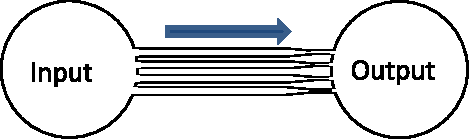
\includegraphics[width=.9\linewidth]{../fig/expdesign1a.pdf}\caption{}\label{fig:expdesign1a}
\end{center}
\end{subfigure}
\begin{subfigure}[b]{0.4\linewidth}
\begin{center}
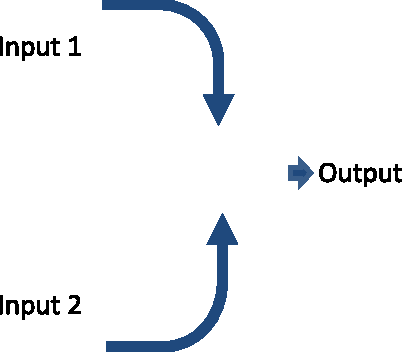
\includegraphics[width=0.5\linewidth]{../fig/expdesign1b.pdf}\caption{}\label{fig:expdesign1b}
\end{center}
\end{subfigure}
\caption{Schematic representation of tapered guidance microfluidic NLDs. The basic Threshold element is depicted in (\subref{fig:expdesign1a}), where the tapered guidance of axons from Input to Output is demonstrated. A limited number of axons cross into the Output, causing only amplitudes that are larger than a given threshold amplitude to be transferred into the Output. In (\subref{fig:expdesign1b}) the principle of combining two of the devices into an AND gate is shown. The columns in the mixing region of the axons, before entering the Input region, allow for a controlled interaction and combination of axons from the two Input regions into the Output region.}\label{fig:expdesign}
\end{center}
\end{figure}

More complex patterns, similar in spirit to the one shown in Figure \ref{fig:nnGeo}, necessitate a number of crossover connections, where axons pass next to or across each other yet do not touch. These will be achieved by patterning an additional layer of microfluidic above the initial pattern, in which the axonal connections (for example from Input 1) can pass over the axons extending from another area (for example from Input 2). Although 3D overlay has not been used to date in neuronal cultures and is technically more demanding, the principles underlying its use and the technology \cite{Rotem2012} itself are similar to the standard 2D patterning that is used in our laboratory.
An innovative aspect of the theoretical design in Figure \ref{fig:expdesign2}, which has not been emphasized to date in the construction of NLDs, is the existence of multiple regions that serve as alternate Output areas. In particular this answers the need, raised in the theoretical part of this proposal, to differentiate the various Input patterns by the ability of the NLD to process them. Be it due to their temporal sequence or their spatial form, there will typically be a large set of Inputs that a given NLD is unable to process. In such cases we would like the NLD to classify the Input as ‘unsuitable’ for processing, and yield an ERROR message at its Output. We would thus expect a large number of input configurations to flow into this ‘nonsense Input’ bin, which is in fact what any competent information processing or computation system must be able to do.
In addition, we expect to utilize ‘temporal patterning’, an important addition to our existing ‘spatial patterning’ effort, to a greater degree and to rely on this novel approach more in the construction of NLDs. By controlling the sequence of seeding of neurons inside the NLD, we have already been able, in preliminary experiments, to get behavior that is very different from regular, same-time NLDs. This approach relies on the fact that neurons taken from embryonic rats or mice are promiscuous in their connections to other neurons from a different animal, a property that does not exist in the living animal where the immune system is expected to play an important role in allowing such connectivity (though this is overcome in our lab by the use of siblings from the same litter).

As in any successful experimental design effort, we expect a continuous back-and-forth process between the lab and the theory, with ideas for novel implementations of NLDs stemming from the theoretical, fundamental considerations being tested out in the lab. This will serve as an immediate reality check (within the limitations of experimental time scales, of course) for the conceptual ideas. Both the ability to construct such NLDs and the actual function in practice versus that predicted will be monitored in this way. We expect this type of collaboration of theory and experiment to be extremely conducive to obtaining efficient NLDs on one and deep insight into fundamental issues of biological computation on the other. 

\subsection{Higher-Order NLDs}
The natural extension of the simple NLDs we have built is the addition of complexity to the network structures. Looking at our current technology, the basic one dimensional structure is designed as a feed-forward device, where the flow of information is linear and directed. Activity originates at Burst Initiation Zones [1], and propagates from there along the linear configuration of the network. In the simplest current experimental one dimensional construction, axons propagate both forward and backwards and connections can go in both directions. This implies that some recurrent connectivity is already a part of the simple linear structures that we have built. However, once we realize that the neuron that has fired has a delay time before it can fire again, we realize that the role of loops is small [2]. In particular, almost all feedback activity is eliminated in the Diode construction [3], which allows axons to go with strong preference in one direction. Using this engineering approach, we have built an oscillator with one closed circuit [3], which relies on the Diode construct and inherently disallows feedback activation. This drives the system into the basin of attraction of a limit cycle, and we have produced a periodic oscillation in this manner.

The next level of complexity is that of networks which incorporate loops, and allow feedback as well as feed-forward activation, both processes that are of importance in the brain [4]. In general for our experimental network, the fundamental object is the relation between two nodes, or a connection of two neurons. The simplest structure that describes such a network theoretically is the tree-like graph, which ignores the possibility of any connections looping back to create a closed circuit. Since a tree-like structure is more tractable analytically, many theoretical approached utilize it. A deviation from the tree structure involves the creation of loops.

In a random graph the probability for closing a small, three node triangular loop is small [5], but in real world networks [6] the appearance of loops is the standard rather than a rarity. Loops in the neurobiological context imply the existence of recurrent connections, which are assumed to be highly represented in the brain, linking brain levels that interact both directly and inversely. This is presumably crucial for several forms of computation, in particular models combining both top-bottom and bottom-up processes in the brain. 

The approach we are proposing is based upon the relation of structure and function in the computational ensemble or organism. Loops are the dominant and characteristic sub-structure and carry most of the functionality in many complex webs and network [7]. To incorporate loops that allow transfer of information both back and forth, we plan to introduce two experimental configurations, both of which depend on constructing the network from a few subsets of neurons that interact.

The first construct is based on our ability to separate different parts of the network in space, and to control the direction of connectivity between them.  It has been shown that by patterning a network so that different areas are active separately, a non-trivial array of interesting oscillatory activity can be observed [8]. The simplest experimental design is one in which several patches are situated on a circle comprised of a thin line along Diode structures are created. Neurons are seeded on the patches, and their axons first interact within the patch, and then propagate out, in the one direction that the Diode allows. This is exemplified in the simple schematic of Figure 1, which is reminiscent of a neuronal construction [9] that has been shown to support recurrent and persistent neuronal activity.

\begin{figure}
\begin{center}
\begin{subfigure}[b]{0.24\linewidth}
\begin{center}
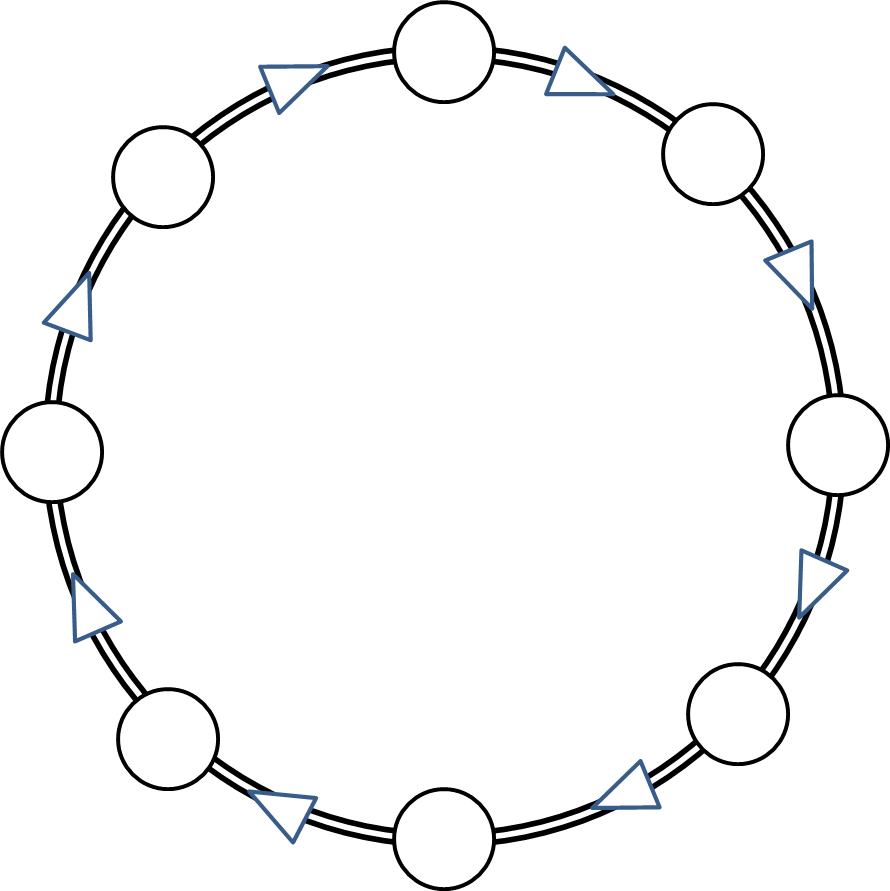
\includegraphics[width=0.7\linewidth]{../fig/expdesign2.png}\subcaption{}\label{fig:expdesign2}
\end{center}
\end{subfigure}
\begin{subfigure}[b]{0.24\linewidth}
\begin{center}
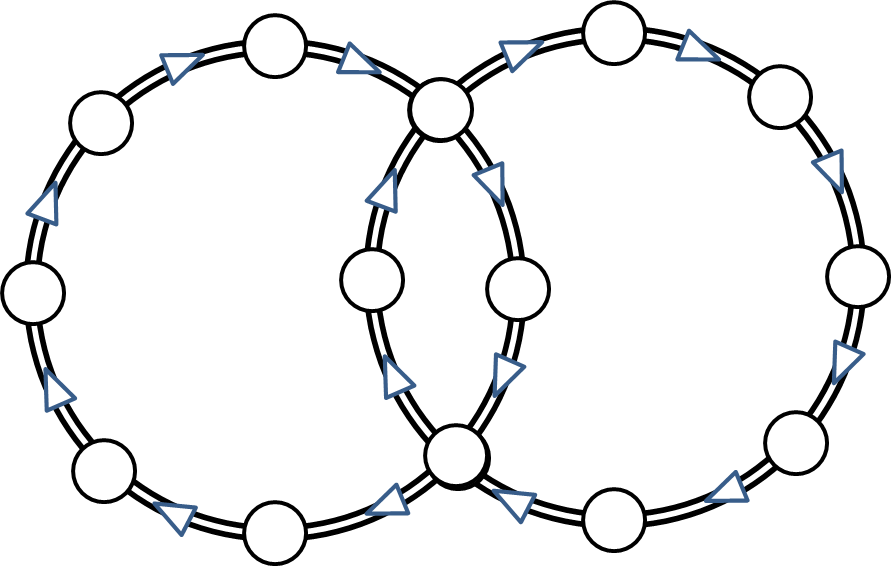
\includegraphics[width=\linewidth]{../fig/expdesign3.png}\subcaption{}\label{fig:expdesign3}
\end{center}
\end{subfigure}
\begin{subfigure}[b]{0.24\linewidth}
\begin{center}

\includegraphics[width=\linewidth]{../fig/expdesign4.png}\subcaption{}\label{fig:expdesign4}
\end{center}
\end{subfigure}
\begin{subfigure}[b]{0.24\linewidth}
\begin{center}
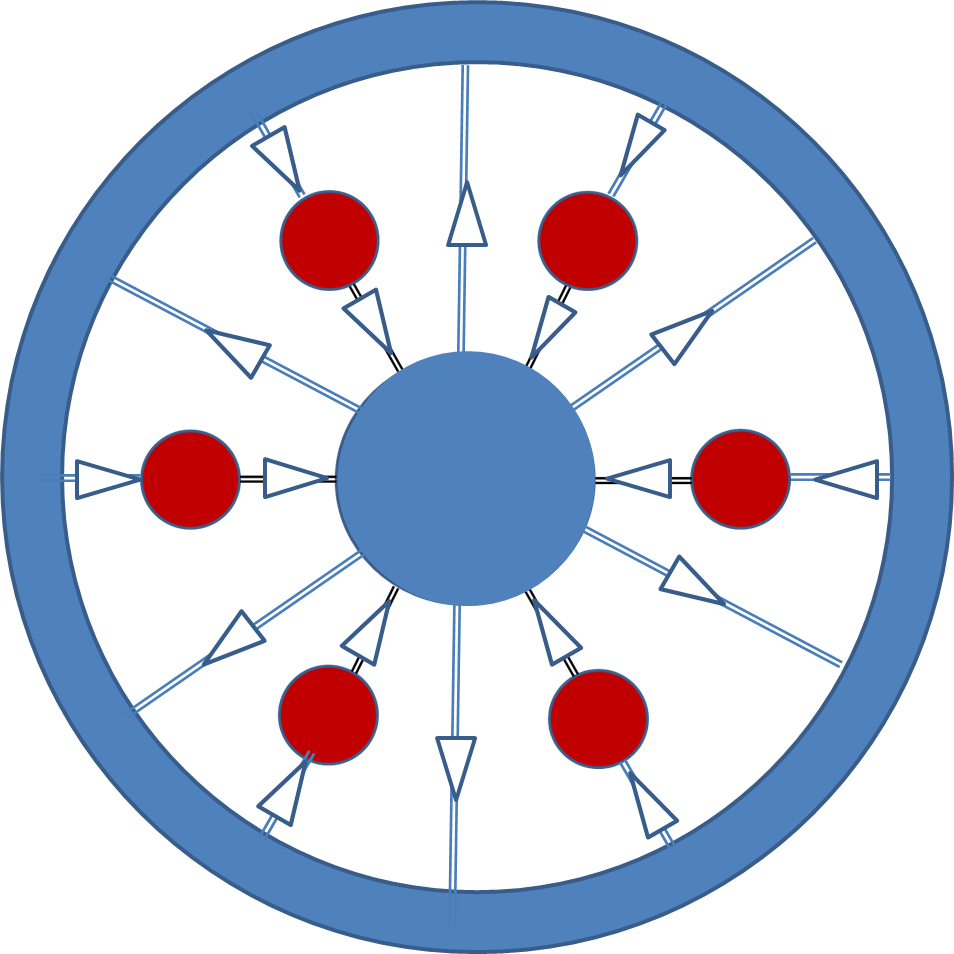
\includegraphics[width=0.7\linewidth]{../fig/expdesign5.png}\subcaption{}\label{fig:expdesign5}
\end{center}
\end{subfigure}
\end{center}
\caption{(\subref{fig:expdesign2}) Schematic of an 8-length loop device in which several sub-networks interact in a uni-directional, ordered mode. Neurons are seeded on the circular areas. After an initial growth period in which axons connect to neurons within the circle, axons will begin to propagate in the direction dictated by the Diode structure. This enforces a directional connection between the sub-networks. (\subref{fig:expdesign3}) The simple doubling and reconnection of an 8-length loop device creates several new loops of differing lengths. The dynamics is hard to predict {\it a priori}, but will present an excellent testing ground for theoretical approaches and models of computation. (\subref{fig:expdesign4}) Schematic diagram of a uni-directional link between two types of neuronal populations. For example, in this particular configuration, the blue culture could be comprised of sensory neurons taken from the peripheral nervous system, while the red culture indicates neurons taken from the central nervous system. (\subref{fig:expdesign5}) Schematic diagram of a loop incorporating the two types of neuronal populations. Here the time sequence is controlled by the Diode links between the cultures, which can serve as significant delay lines. The relative size of the different areas must be}
\end{figure}

It is straightforward to see that this kind of loop structure can be generalized, and that the ensuing dynamics will display a wide variety of fascinating nonlinear behavior. The configuration shown in Figure \ref{fig:expdesign3} demonstrates that just by repeating the same 8-length loop structure and reconnecting, three new loops are created, of lengths 4, 6 and 6, along with a longer loop consisting of 14 nodes. The different time scales associated with propagation in each of the different loop lengths ensures that the dynamics will be intriguing.

The second experimental configuration we intend to employ is that of combining two different neuronal populations that will interact with each other. This is an exploratory attempt, and we will have to experiment with a variety of different neuronal types. The idea is simply depicted in Figure \ref{fig:expdesign4}, where one type of neuronal network is feeding into a second type.

This basic configuration assumes that one type of neuronal culture is more typically an output provider, for example the sensory neurons from the peripheral nervous system (PeNS) in the body that typically send their output into the central nervous system (CNS). Closing the loop is such a system can be done in a number of interesting patterns, for example the configuration of Figure \ref{fig:expdesign5}. Note that the thin lines linking the different nodes provide a delay line, so that there is a temporal sequence superimposed on the spatial pattern.

Several technical challenges arise in this project. First, the seeding of different neuronal types implies that microfluidic devices are the system of choice. Feeding channels can convey the neurons into the respective areas for either neuron along separate channels that can reside in a feeding layer that is separated vertically from the culturing layer. Second, the choice of neuronal types is a matter for continual exploration. While the harvesting of peripheral neurons is simple, their interaction with the CNS neurons is far from predictable, and the results from such a co-culture are not known. We also plan to separate different types of population using genetic parking and a fluorescent activated cell sorting (FACS) machine. While this is clearly feasible, the separation procedure will necessarily introduce a delay on the order of an hour between the harvesting of the cells and seeding. It remains to be seen whether this will impact the survival of the neuronal types.

The introduction of several different neuronal networks made of different neuronal types that communicate, interact and feedback onto each other addresses a deep problem of the self-assembly of computation in living neuronal networks. The failure of a cultured neuronal network to produce a valid computation is associated with the fact that it is grown out of context, out of its natural surroundings. We have shown that geometrical constraints can coax some of the networks connections to go in preferred directions, restoring a modicum of computation [3]. However, in fact the neurons are growing out of their natural context, and the input that they are exposed to during the growth process is not the one that naturally leads them to advance a significant computation. We could say that there is a `software' growing inside the network, but that this software does not have the needed input from its hardware to guide it towards a ‘meaningful program’. 

The plan to co-culture different sets of neurons along with the regular hippocampal ones is thus the natural solution and a first step in creating a ‘hardware-software’ linkage in a neuronal culture. The first choice is that of sensory neurons, since those are the subset of neurons that communicate between the body of the organism and its brain. In this way we hope to recreate an information channel that exists in the developing brain, allowing neurons to attain functional connectivity according to the inputs it receives.

The general theoretical relevance of loops to the construction of computation will lead us to address the issue of self-reference in computational systems, a problem that is both deep and stimulating [10]. From the point of view that identifies the capacity for abstraction with computation, the investigation of neuronal logic devices capable of such function provides a framework in which various hypotheses from cognitive science could begin to be evaluated at the level of well-defined neural circuits. By attempting to isolate minimal implementation criteria, this approach may serve to complement, enable simpler explanations of, or identify paradoxical results derived from studies that treat whole brains and their associated sensory apparatus as their object of study [11,12].

\subsection{ANN simulation of abstract computation in NLDs}
In order to facilitate the formation of a simple higher-order boolean function capable of switching between the AND and OR gate ($\wedge / \vee$) functionality as a result of the growth of patterned cultures of neurons, we designed a potential geometric constraint shown in Figure \ref{fig:nnGeo} to use in simulations of neural network development. We implemented one potential impact upon network connectivity in terms of an artificial neural network (ANN) model. Figure \ref{fig:hintDiag} shows Hinton diagrams for the weights of 3-input 3-layer 1-output feedforward ANNs trained on data representing the $\wedge / \vee$ gate switching task and selected for near perfect performance on this task. Figure \ref{fig:nnDendro} shows a heatmap where neural networks are clustered according to their respective weights in order to determine the degree to which networks capable of performing the $\wedge / \vee$ gate switching task may be clustered into a reduced number of strategies despite the apparent diversity demonstrated in Figure \ref{fig:hintDiag}. We see from Figure \ref{fig:nnDendro} that, while there is considerable diversity in the 50 networks sampled in our simulations, there are also relative similarities between neural network designs that are all approximately equivalent in terms of their capacity to perform $\wedge / \vee$ gate switching.

\begin{figure}
\begin{center}
\begin{subfigure}[b]{0.45\linewidth}
\begin{center}
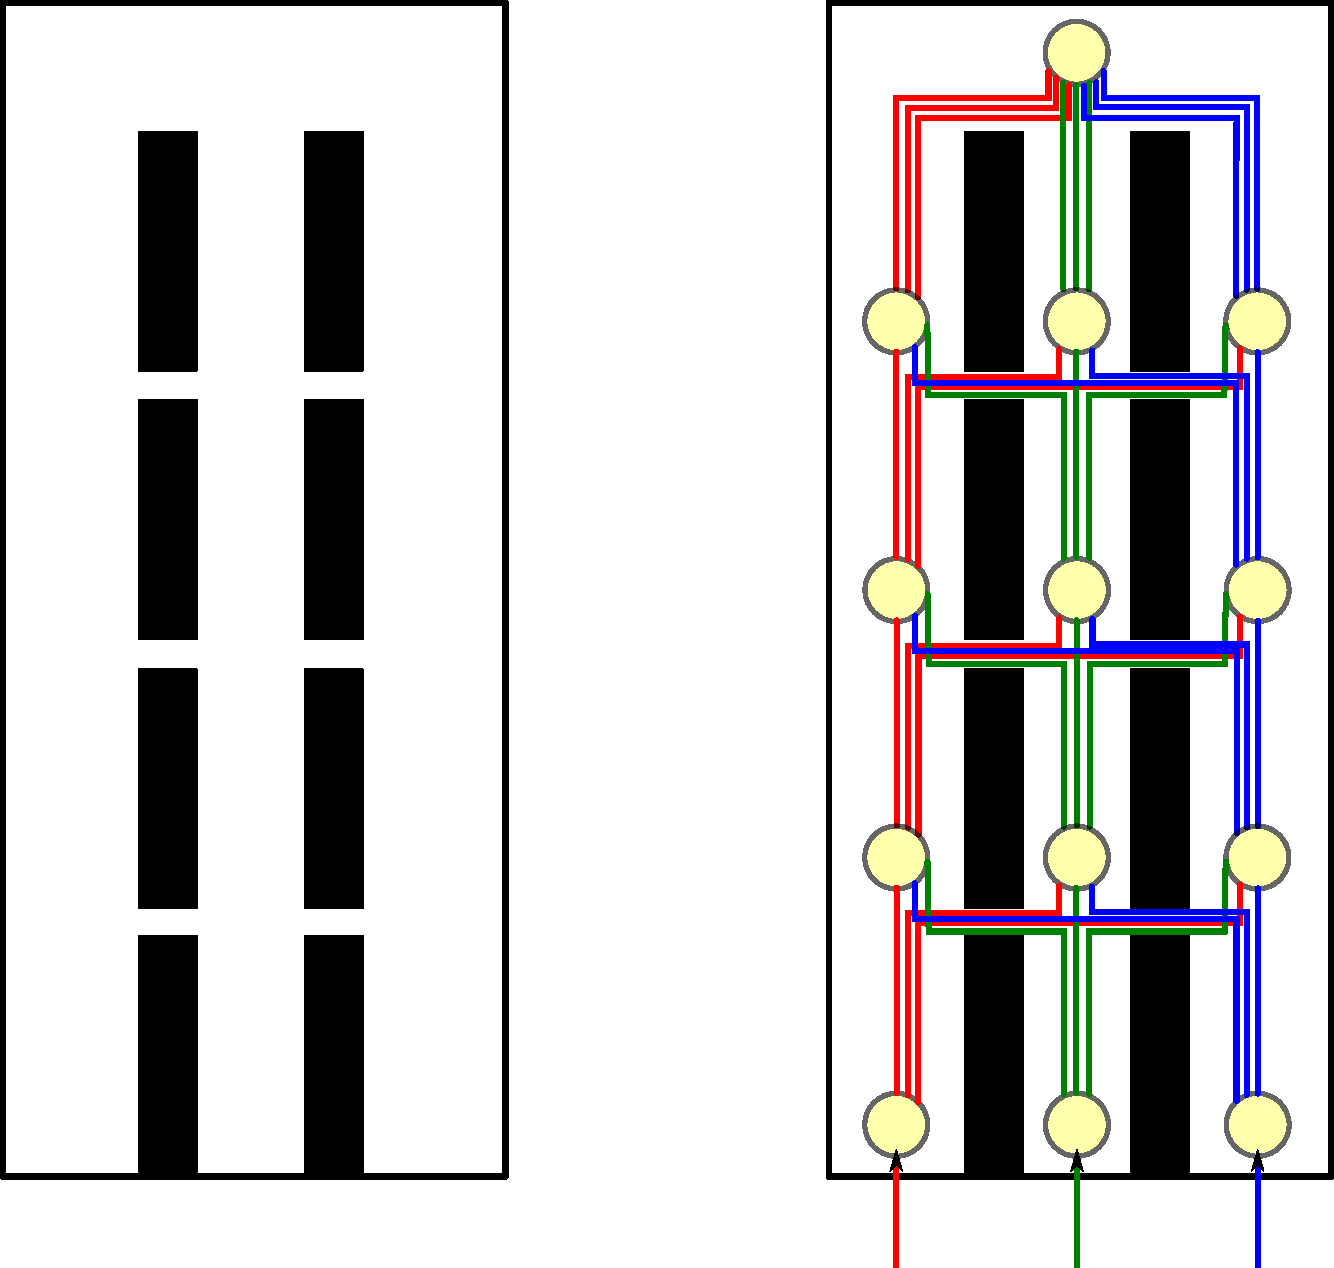
\includegraphics[width=.65\linewidth]{../fig/aogeometry.pdf}\caption{}\label{fig:nnGeo}
\end{center}
\end{subfigure}
\begin{subfigure}[b]{0.45\linewidth}
\begin{center}
\begin{tabular}{cccc}
{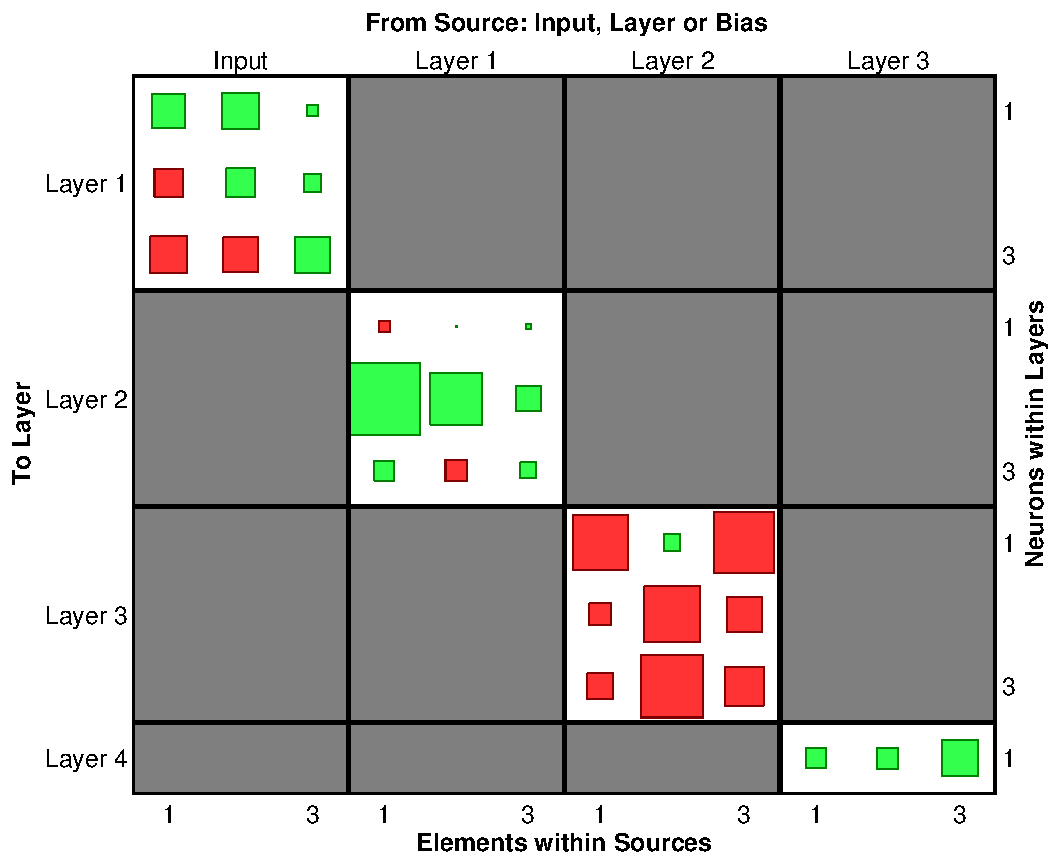
\includegraphics[width=0.2\textwidth,page=1]{../fig/combined.pdf}} 
   & {\includegraphics[width=0.2\textwidth,page=2]{../fig/combined.pdf}}
   & {\includegraphics[width=0.2\textwidth,page=3]{../fig/combined.pdf}} 
   & {\includegraphics[width=0.2\textwidth,page=4]{../fig/combined.pdf}}\\
{\includegraphics[width=0.2\textwidth,page=5]{../fig/combined.pdf}} 
   & {\includegraphics[width=0.2\textwidth,page=6]{../fig/combined.pdf}}
   & {\includegraphics[width=0.2\textwidth,page=7]{../fig/combined.pdf}} 
   & {\includegraphics[width=0.2\textwidth,page=8]{../fig/combined.pdf}}\\
{\includegraphics[width=0.2\textwidth,page=9]{../fig/combined.pdf}} 
   & {\includegraphics[width=0.2\textwidth,page=10]{../fig/combined.pdf}}
   & {\includegraphics[width=0.2\textwidth,page=11]{../fig/combined.pdf}} 
   & {\includegraphics[width=0.2\textwidth,page=12]{../fig/combined.pdf}}
\end{tabular}
\end{center}
\caption{}\label{fig:hintDiag}
\end{subfigure}
\end{center}
\caption{(\subref{fig:nnGeo}) Theoretical geometric constraint facilitating the formation of the $\wedge / \vee$ gate switch. The geometric constraint is shown on the left and the artificial neural network wiring diagram representing potential connections whose strength is modulated upon training of the network is shown on the right. (\subref{fig:hintDiag}) Hinton diagrams of feedforward neural network weights for neural networks trained on the and/or gate switching task.}\label{fig:neuralnets}
\end{figure}

\begin{figure}
\begin{center}
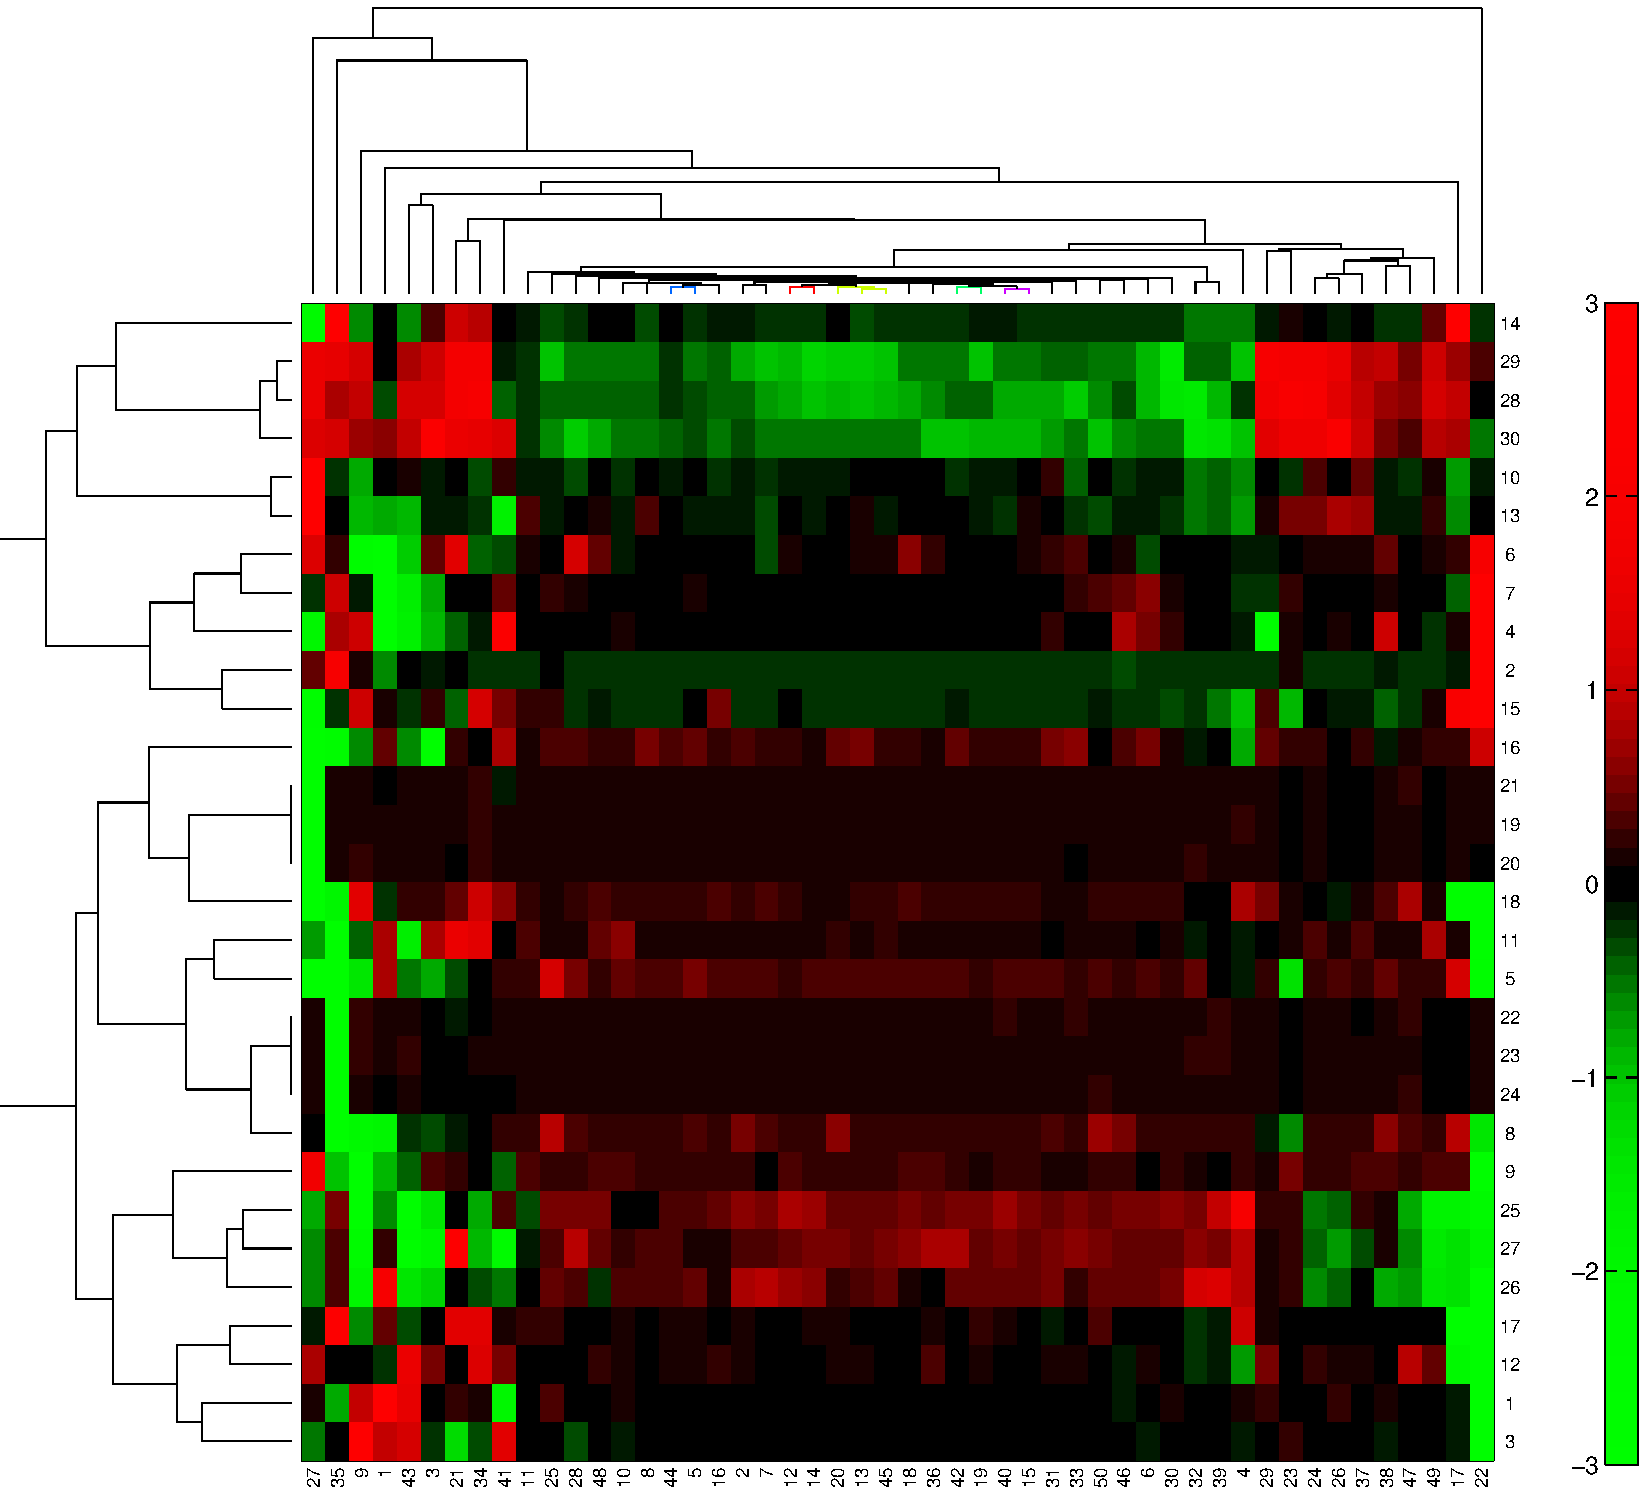
\includegraphics[width=0.25\textwidth]{../fig/dendrogram.pdf}
\end{center}
\caption{Theoretical geometric constraint facilitating the formation of the $\wedge / \vee$ gate switch. A heatmap that is clustered along rows representing individual weights at particular positions within the ANN and along columns according to the ANN from which the weights derive showing the relationship between low error strategies that emerge in training 50 independent ANNs on the $\wedge / \vee$ gate switching task.}\label{fig:nnDendro}
\end{figure}

\subsection{From NLDs to the CNS and principles of cognition}

As noted above, we associate the failure of a cultured neuronal network to produce a valid computation with the fact that it is grown out of context, out of its natural surroundings. By using geometric constraints, we have shown that we can coax some of the networks connections to go in the direction we engineer, and a modicum of computation is restored \cite{Feinerman2008}. However, the idea that the `software' is growing without the presence of the `hardware' it is accustomed to, leads us to the idea of co-culturing a different set of neurons along with the regular hippocampal ones. The obvious choice for us is that of sensory neurons, since those are the subset of neurons that communicate between the body of the organism and its brain. In this way we hope to recreate an information channel that exists in the developing brain, allowing neurons to attain functional connectivity according to the inputs it receives.
We are thus communicating with a number of groups that study pain, with the intention of extracting sensory neurons that synapse onto CNS neurons to convey the signals associated with stress and pain. This is a natural initial choice, since the preception of pain signals is fundamental to survival in many cases and thus neurons may have evolved to be robustly sensitive to such signals.

From the point of view that identifies the capacity for abstraction with
computation, the investigation of neuronal logic devices capable of such
function provides a framework in which various hypotheses from cognitive
science could begin to be evaluated at the level of well-defined neural
circuits. By attempting to isolate minimal implementation criteria, this
approach may serve to complement, enable simpler explanations of, or
identify paradoxical results derived from studies that treat whole
brains and their associated sensory apparatus as their object of study
\cite{McClelland2010,Griffiths2010}.

\section{Section 4: Role and expertise of the PIs}
Both Profs. Aviv Bergman and Elisha Moses have significant experience working in collaborative teams of experimentalists and theorists. The PIs intend this project to involve strong interaction between experiment and theory. Prof. Bergman will lead the theoretical component of this project. Prof. Bergman's expertise spans a number of theoretical areas including artificial neural networks, dynamical systems, mathematical evolutionary biology, and systems biology. The Bergman lab will develop the computational platform and analytical tools to predict neuronal architecture-function relationships, which in turn will help guide the construction of environmental conditions to guide the development of natural neural networks capable of performing fundamental computational tasks. Prof. Moses will lead the experimental component of the project, heading a laboratory that focuses on the growth and measurement of neuronal activity in networks grown from CNS neurons from rat and mouse brain. The lab has pioneered the design of complex neuronal logical devices, has generated several new experimental paradigms combining nonlinear dynamics and statistical physics with biological physics, and has participated in the formation of novel theoretical models for engineered neuronal networks.

\section{Section 5: Educational involvement}
In the Bergman lab, three Ph.D. students (Mr. Cameron Smith, Mr. Daniel Biro and Mr. Ximo Pechaun) will be involved in developing the theoretical aspect of this project in close interaction with the PI. In the Moses lab two students (1 Ph.D., Ms. Shani Stern and 1 M.Sc., to be hired) and a postdoctoral fellow (Dr. Yaron Penn) will be involved. Students and postdoctoral fellows in the Bergman and Moses labs will interact on a weekly basis via video conference. More extensive interaction will be fostered by an exchange program that we plan to engage in at crucial theory-experiment integration stages throughout the project. Virtual interaction among all involved, including the public, will be fostered by an open online \href{http://en.wikipedia.org/wiki/Wiki}{Wiki} that will be used to organize and collaborate on this project and, more generally, support the movement for \href{http://en.wikipedia.org/wiki/Open\_notebook\_science}{Open Notebook Science}. All computer code will be made open source in accordance with the \href{http://opensource.org/licenses/MIT}{MIT license} and the codebase history will be available to the public free and in real-time on \href{http://www.github.com}{github}. Despite the fact that both labs already combine theory and experiment, they do so in very different ways and exposure to each of these models for combining theory and experiment will be crucial for these students as they move on to make very important decisions in their careers with respect to postdoctoral training and ultimately building labs of their own.